\documentclass{ctexart}
\usepackage{listings}
\usepackage{xcolor}
\usepackage{caption}
\usepackage{graphicx}
\usepackage{float}
\usepackage[colorlinks,
linkcolor=red,
anchorcolor=blue,
citecolor=green
]{hyperref}
\title{操作系统课程设计实验报告}
\author{宋振华}
\date{学号: 201605301357}
\begin{document}
\maketitle
\section{简述}

\subsection{Linux简述}
Linux操作系统是UNIX操作系统的一种克隆系统. 它诞生于1991年, 此后借助于Internet网络, 现已成为当今世界上使用最多的一种UNIX类操作系统, 并且使用人数还在迅猛增长.

Linux操作系统的诞生、发展和成长过程依赖于以下5个重要支柱: UNIX操作系统、MINIX操作系统、GNU计划、POSIX标准和Internet网络. 

通过阅读Linux早期内核版本的源代码, 是学习Linux系统的一种行之有效的途径, 并且对研究和应用Linux嵌入式系统也有很大帮助.

正如Linux系统创始人在一篇新闻组投稿上所说的, 要理解一个软件系统的真正运行机制, 一定要阅读其源代码(RTFSC). 系统本身是一个完整的整体, 具有很多看似不重要的细节存在, 但是若忽略这些细节, 就会对整个系统的理解带来困难.

目前的Linux内核源代码量都在几百万行的数量上, 极其庞大, 对这些版本进行完全注释和说明几乎是不可能的, 而0.11版内核不超过2万行代码量, 麻雀虽小, 五脏俱全.

\subsection{实验目的}
该实验以Linux0.11为例帮助学生探索操作系统的结构、方法和运行过程, 理解计算机软件和硬件协同工作的机制. 学生需要完成4项任务:
\begin{enumerate}
	\item 分析Linux0.11系统源代码, 了解操作系统的结构和方法. 
	\item 通过调试、输出运行过程中关键状态数据等方式, 观察、探究Linux系统的运行过程. 
	\item 建立合适的数据结构, 描述Linux0.11系统运行过程中的关键状态和操作, 记录系统中的这些关键运行数据, 形成系统运行日志. 
	\item 用图形表示计算机系统中的各种软、硬件对象, 如内存、CPU、驱动程序、键盘、中断事件等等. 根据已经产生的系统运行日志, 以动画的动态演示系统的运行过程. 
\end{enumerate}

\section{阅读源码}
\subsection{思维导图}
在阅读源码的过程中, 我利用XMind 8思维导图工具, 将Linux 0.11结构, 绘制成一张静态的思维导图, 以加深对Linux0.11内核各部分的理解. \footnote{思维导图源码见\url{https://github.com/sfd158/oldlinux-homework/blob/master/linux0.11_v1.0.xmind}}
\begin{figure}
	\centering
	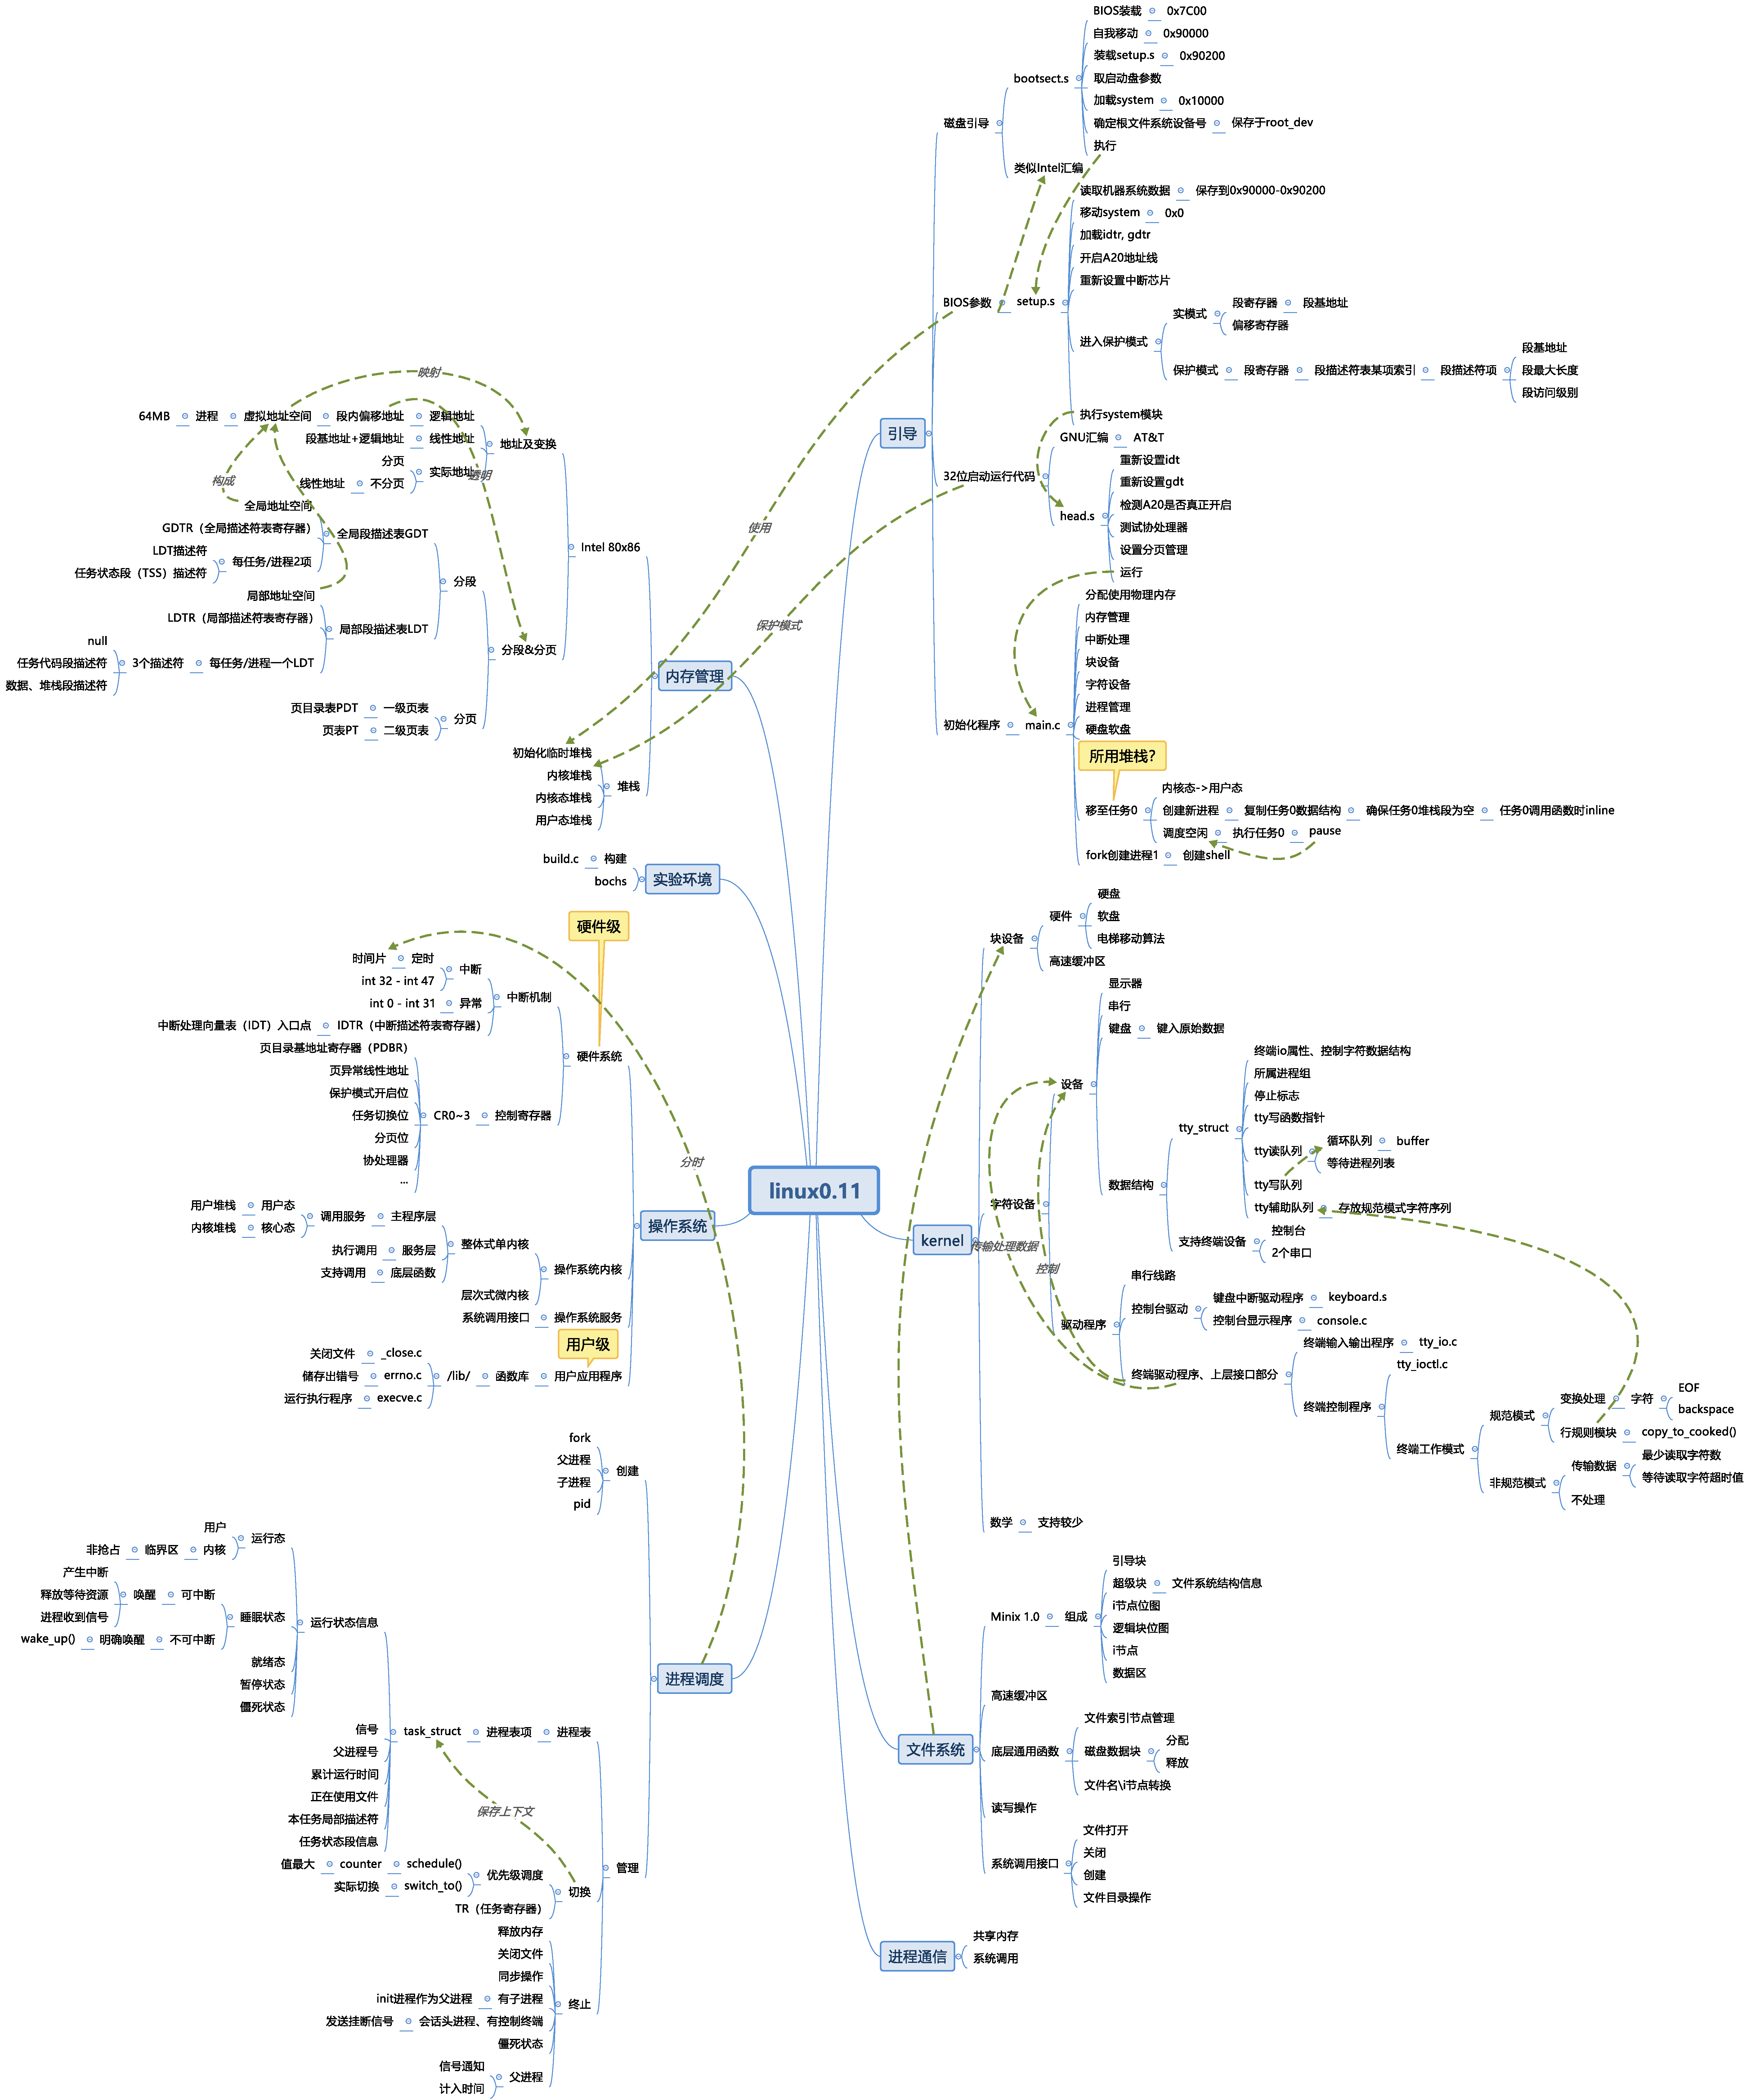
\includegraphics[width=\textwidth,natwidth=2722 ,natheight=3249]{img/linux0.11.pdf}
	\caption[]{linux0.11思维导图}
	\label{fig:linuxgraph}
\end{figure}

\subsection{源码理解}
以下是部分源码理解概述, 更详细的源码理解, 请参考我的Github网站\footnote{\url{https://github.com/sfd158/oldlinux-homework/blob/master/html/explains.json}}.
\subsubsection{引导/启动/初始化}

\paragraph{引导器——bootsect.s}

将全部linux内核载入内存, 跳转至setup.s执行.

\paragraph{初始化CPU和其他硬件——setup.s}

获取系统信息, 初始化CPU和其他硬件. 

\paragraph{初始化c语言运行环境——head.s}

进一步设置CPU和内存, 使得可以直接运行C语言编译好的程序. 

\paragraph{初始化内核功能——main.c}

初始化内核的所有模块和功能, 创建idle进程, 调用shell程序. 

\subsubsection{运行}

\paragraph{系统调用}

向用户程序提供系统调用接口, 是一个操作系统内核所必须具有的功能. 在include/unistd.h中列出了所有(72个)系统调用号, 用户程序通过使用int 0x80指令调用这些系统调用. 大部分系统调用是对文件的操作, 只有少部分涉及退出、返回等. 

\paragraph{内存管理}

内存管理主要靠硬件实现, linux0.11的内存管理代码是配合着80x86的内存管理方案编写的. 

它对外提供的功能有内存的申请和释放, 以及对用户程序运行环境的基本保护. 用户程序通过系统调用可以使用其中部分功能. 

\paragraph{进程调度}

实现了进程的创建、销毁、切换、暂停、唤醒、中断等, 在内核内部使用一个结构体保存了每一个进程的基本信息, 在系统忙时通过时钟中断来实现多任务切换. 

\paragraph{进程通信}

支持内存共享、信号的进程通信方式, 通过特定的系统调用来实现. 

\paragraph{文件系统}

在linux中, 文件系统不仅仅是用来访问存储的. 根据unix的标准, 所有一般硬件都会通过文件系统来抽象成统一的访问接口, 这就使得文件系统的功能非常强大. 

在linux0.11中, 只有两种设备文件:块设备和字符设备, 使用同一个系统调用, 提供了不同的访问方法. 

\section{选择可视化模块}
\subsection{可视化部分}
\begin{enumerate}
	\item 开机启动过程: 统计了开机启动过程中, 所有C语言函数被调用的情况. 
	\item 字符显示过程:
	\subitem 控制台输入echo hello系统的执行情况;
	\subitem 控制台输入a.out(该程序在控制台输出hello,world!)系统的执行情况.
\end{enumerate}
\subsection{提取什么数据}
\begin{enumerate}
	\item 对于开机启动过程, 当每个C语言函数被执行到时, 输出调用栈, 以观察调用、被调用情况.
	\item 对于字符设备, 当每个C语言函数被执行到时, 输出调用栈, 以观察调用、被调用情况; 同时当屏幕被修改时, 输出屏幕内容.
\end{enumerate}

\section{可视化方案}

\paragraph{编程语言}
可视化展示界面使用HTML5+JavaScript+CSS3. 优点: 设计界面较为快捷.
\paragraph{实现如下功能:}
\begin{enumerate}
	\item 介绍每个源文件的用途;
	\item 统计启动过程调用信息, 以柱状图形式展现;
	\item 实现字符输出过程的动画, 包括
		\subitem 在终端执行echo hello与a.out;
\end{enumerate}

\subsection{最终效果}
在网页上, 呈现出以下效果: \footnote{可通过\url{http://123.207.166.164:23333/}使用此可视化界面.}
\begin{figure}[htbp]
	\centering
	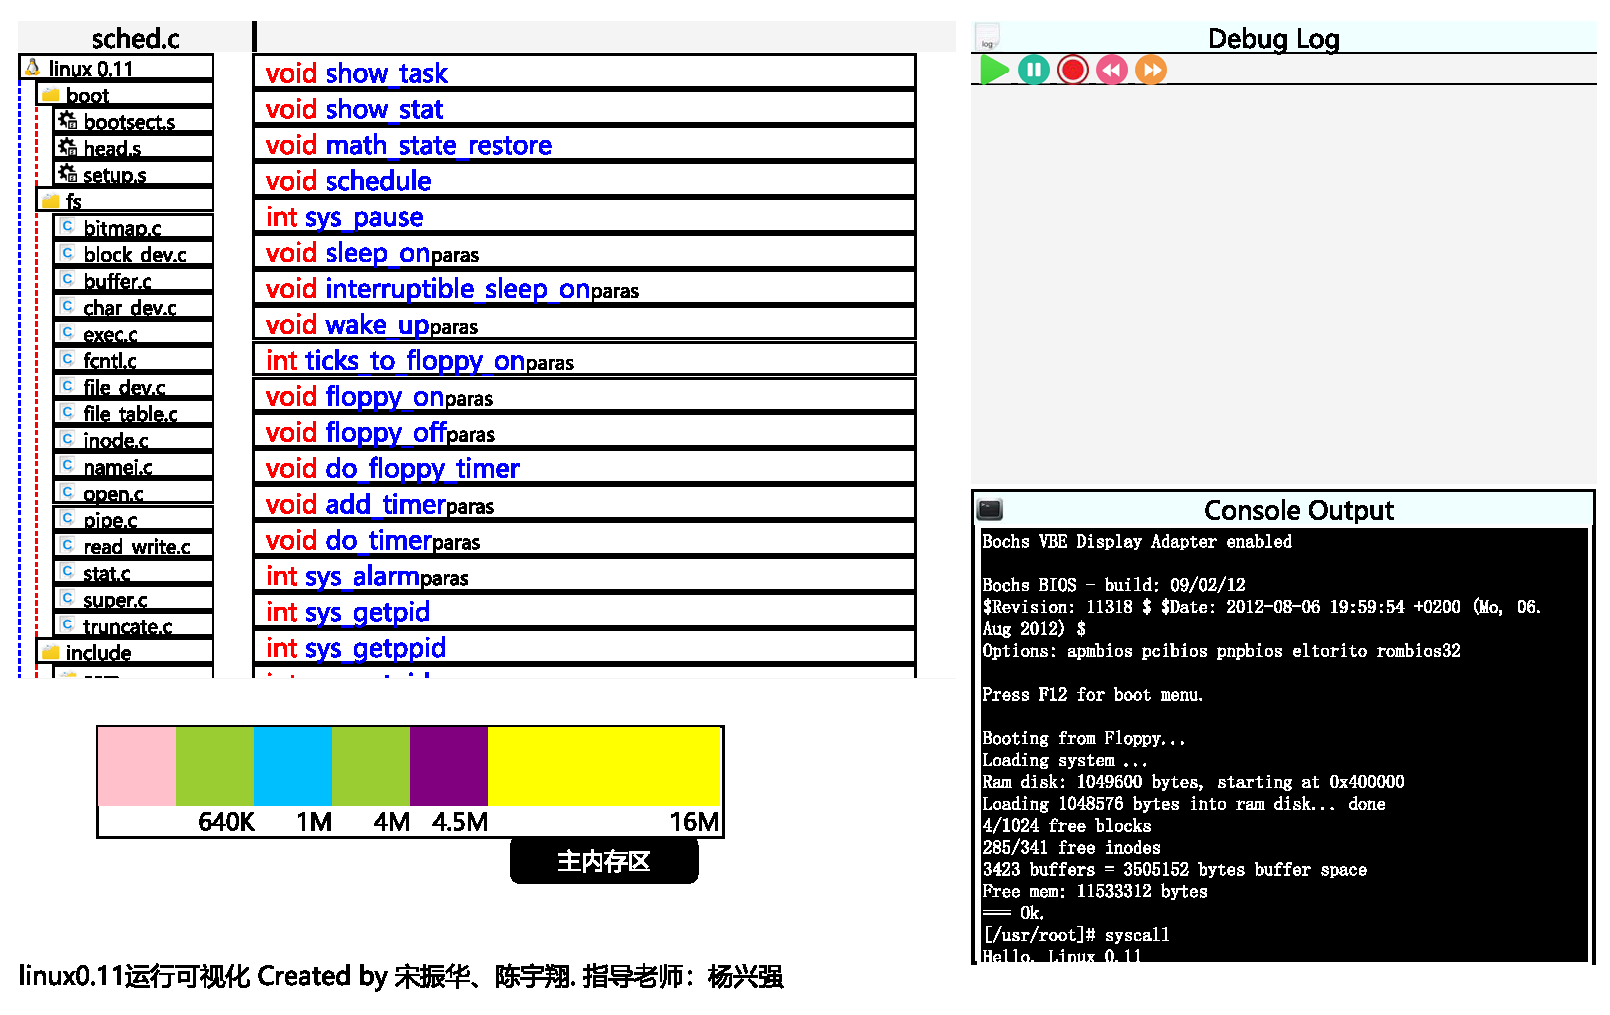
\includegraphics[width=\textwidth,natwidth=773 ,natheight=487]{img/index.html.pdf}
	\caption[]{主页, 包含对每个文件功能的介绍; 模拟内存及console}
	\label{fig:indexgraph}
\end{figure}

\begin{figure}[htbp]
	\centering
	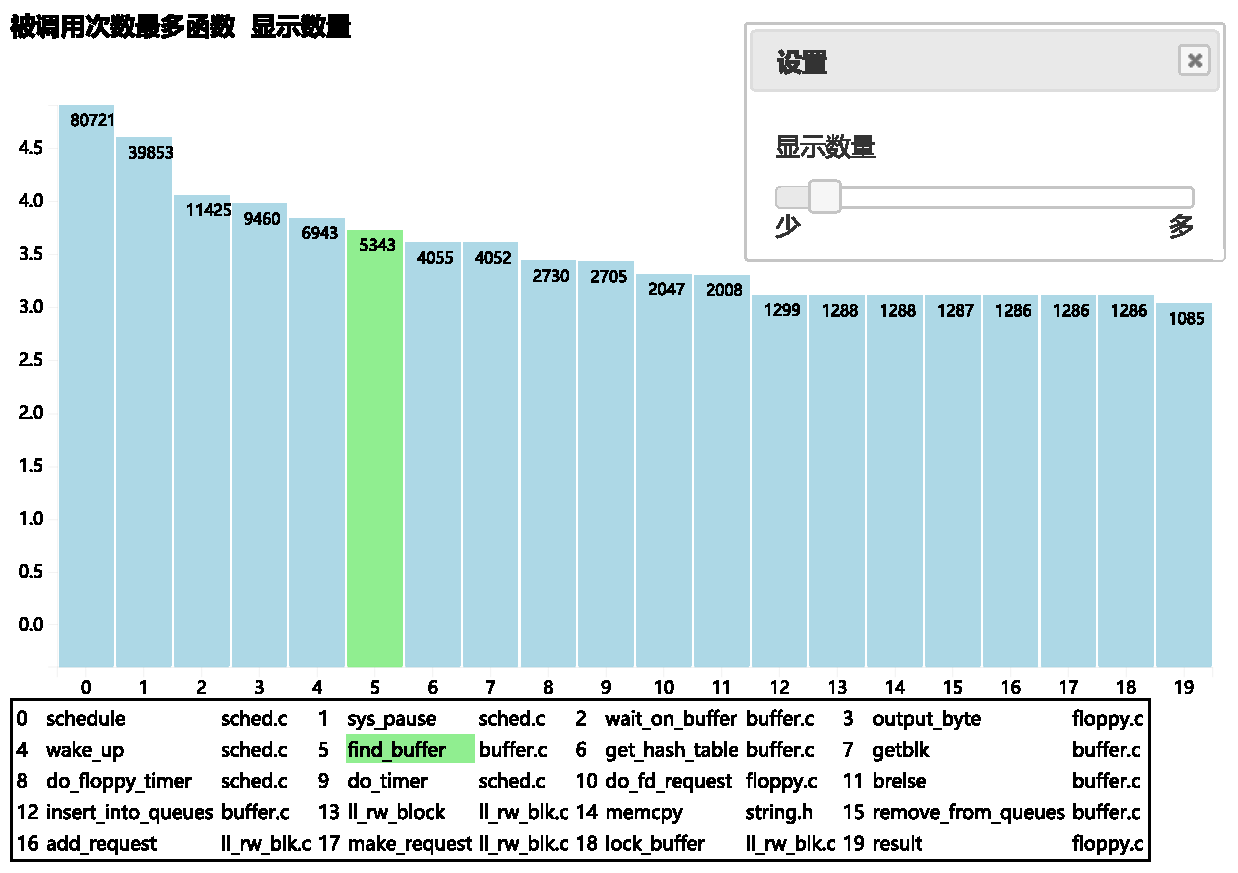
\includegraphics[width=\textwidth,natwidth=594 ,natheight=419]{img/calledMaxFunc.pdf}
	\caption[]{“引导界面调用次数最多”的函数 统计图. 表格与条形图可进行简单的交互. 纵坐标为log坐标轴}
	\label{fig:calledMaxFuncgraph}
\end{figure}

\begin{figure}[htbp]
	\centering
	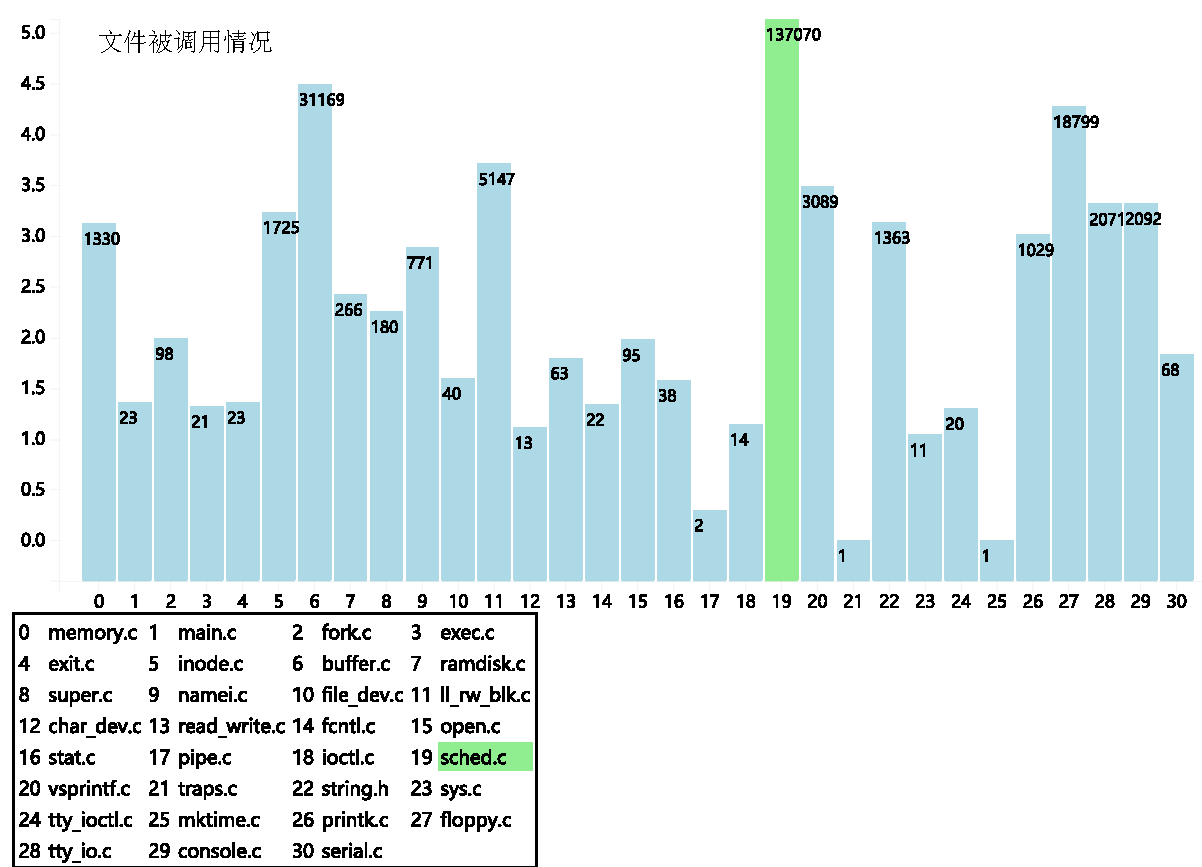
\includegraphics[width=\textwidth,natwidth=577 ,natheight=416]{img/calledFile.pdf}
	\caption[]{“引导界面调用次数最多”的文件 统计图}
	\label{fig:calledMaxFilegraph}
\end{figure}

\begin{figure}[htbp]
	\centering
	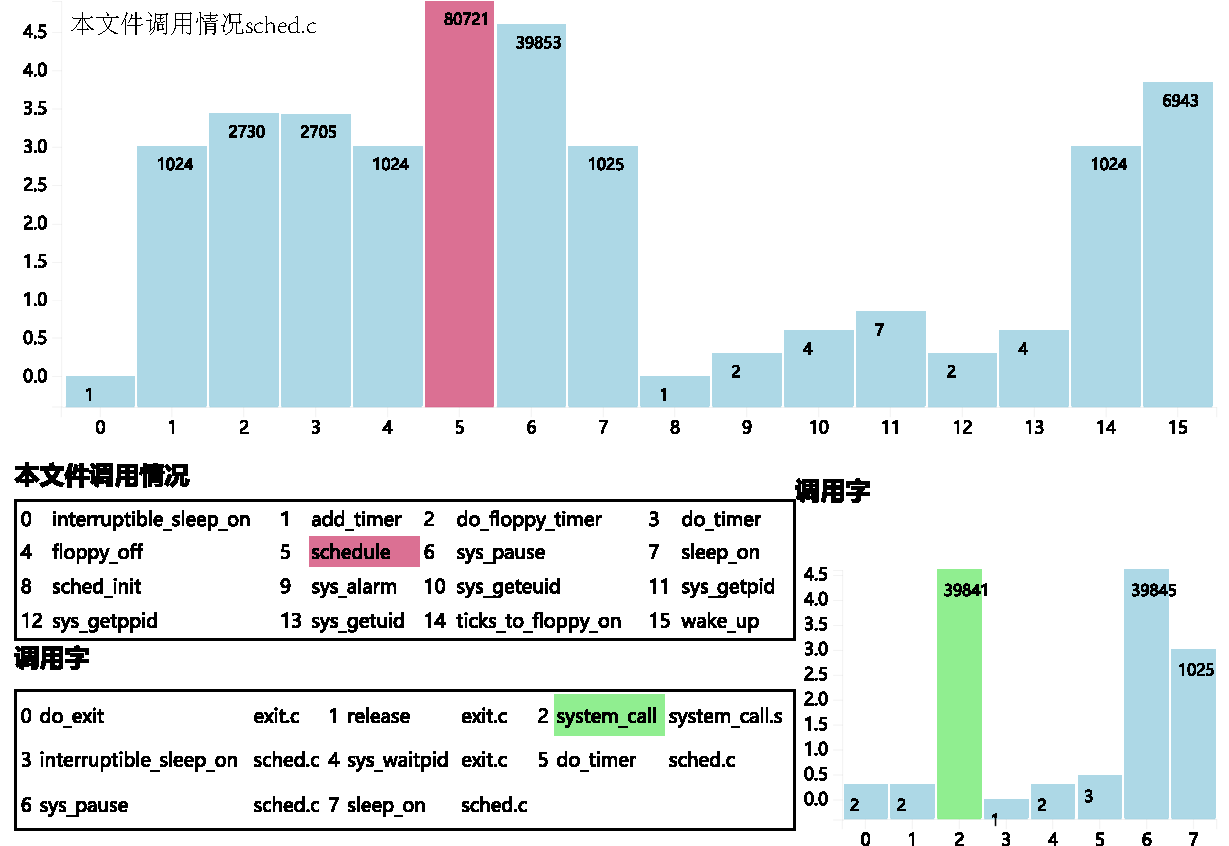
\includegraphics[width=\textwidth,natwidth=590 ,natheight=406]{img/eachFileCall.pdf}
	\caption[]{这是sched.c中函数统计调用图. 点击某函数, 可显示对应的调用字.}
	\label{fig:eachFileCallgraph}
\end{figure}

\begin{figure}[htbp]
	\centering
	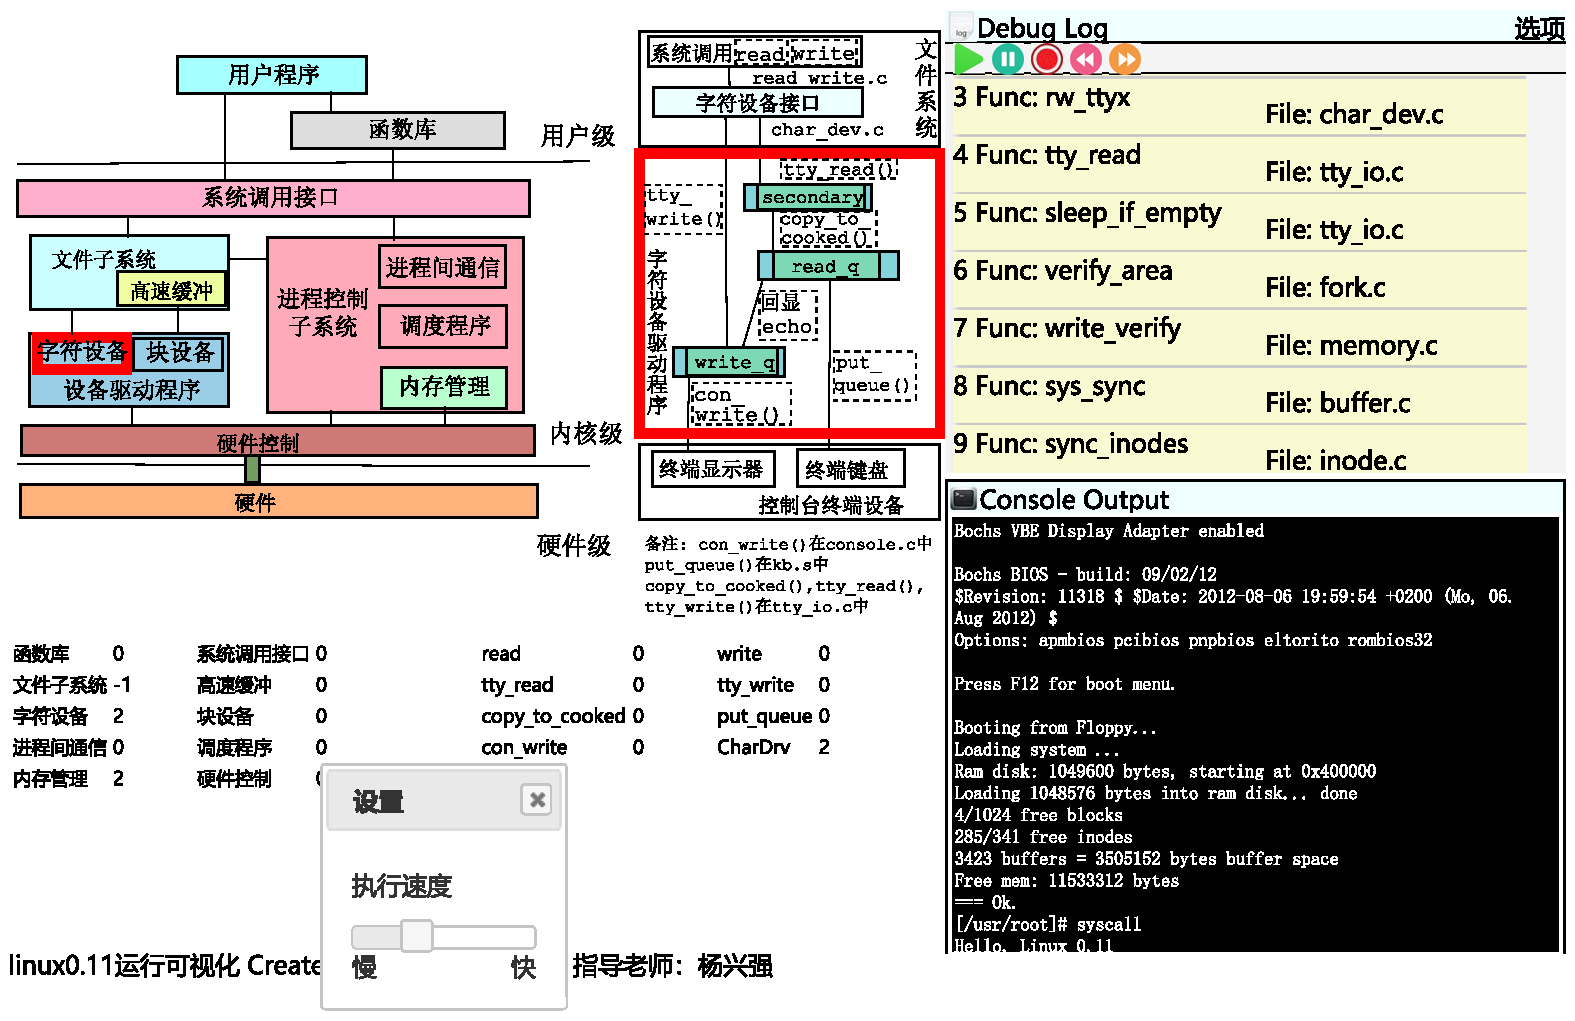
\includegraphics[width=\textwidth,natwidth=756 ,natheight=450]{img/chrdrv.pdf}
	\caption[]{字符设备动图}
	\label{fig:ChrDrvgraph}
\end{figure}

\section{提取数据细节}
\subsection{数据格式}
由于数据极多, 此处只列举输出数据示例. 
\footnote{详细数据和源代码可以查看\url{https://github.com/sfd158/oldlinux-homework}}
\paragraph{文件功能说明}
\begin{lstlisting}[language=HTML]
"bitmap_c":
{
"src":"0.11/fs/bitmap.c",
"brief":"文件系统部分",
"detailed":
"包括对i节点位图和逻辑块位图进行释放和占用处理函数. 
操作i节点位图的函数是free_inode()和new_inode(), 
操作逻辑块位图的函数是free_block()和new_block()"
}
\end{lstlisting}

\paragraph{函数类别说明}
\begin{lstlisting}
{
"verify_area":"MemoryManage",
"write_verify":"MemoryManage",
"rw_char":"CharDrv",
"rw_ttyx":"CharDrv",
"tty_read":"CharDrv",
...
}
\end{lstlisting}
\paragraph{执行过程记录}
\begin{lstlisting}
[
{"funcName":"verify_area", "fileName":"fork.c"},   //调用栈第0层
{"funcName":"sys_read", "fileName":"read_write.c"} //调用栈第1层
]
\end{lstlisting}
\subsection{注意事项}
对于使用gdb脚本调试, 应当注意以下几个方面:
\subsubsection{添加断点}
\paragraph{缺页中断加断点}
在执行过程中, 会频繁访问中断向量表, 或发生缺页中断. 此时gdb会收到一个信号, 并暂停.

\subparagraph{解决方案}
在对应位置添加断点, 让gdb在此处继续执行. 如下:
\begin{lstlisting}
break head.s:19
comm
c
end
break page.s:15
comm
c
end
\end{lstlisting}

\paragraph{断点不宜太多}在gdb脚本中, 不能一次性添加太多断点, 否则会严重影响执行速度. 原因如下:
\begin{enumerate}
	\item 频繁执行gdb脚本, 耗费大量时间在gdb输出, 保存断点等方面;
	\subitem 举例来说, console.c中的所有函数, 在系统启动时, 总计被调用了5000多次.
	\subitem 如果在诸多函数添加断点, 系统启动过程, 断点可能被执行到几十万次.
\end{enumerate}
\subparagraph{解决方案}
如果需要大量记录数据, 可以将大量断点分成若干批次, 每次执行只加入其中一部分断点. 

优点: 每次调试产生的数据量较小. 由于gdb执行时间不影响bochs时钟中断产生次数, 因此不会产生时间片轮转次数大幅增加的误差.

缺点: 不能完全保证两次执行操作完全相同, (如时钟中断时机不一定完全相同).

相比而言, 由于linux具有很好的模块性, 各模块之间耦合性较低, 分别调试问题不大.

\paragraph{加断点需谨慎}

在linux0.11中, 有些函数执行极其频繁, 如sched.c中void schedule(void)函数(该函数用于时间片轮转). 如需要gdb连续地执行代码(区别与单步调试), 这些函数会频繁被执行, 从而严重影响速度. 原因同上.

有些函数定义后, 从未被使用, 在编译时这些函数会被自动优化掉. 如include/string.h中memmove, memcmp, memchr函数. 如果在这些函数上添加断点, gdb会在别的位置暂停, 或是崩溃.

\paragraph{汇编语言添加断点}
汇编语言中定义的函数, 类似于这样:
\begin{lstlisting}
keyboard_interrupt:
pushl %eax
pushl %ebx
pushl %ecx
pushl %edx
push %ds
push %es
movl $0x10,%eax
mov %ax,%ds
mov %ax,%es
xor %al,%al		/* %eax is scan code */
inb $0x60,%al
cmpb $0xe0,%al
\end{lstlisting}
其中keyboard\_interrupt为函数入口, 随后几条pushl等语句, 为函数参数初始化过程. 调试汇编时, 汇编文件中不是所有的行都会执行, 比如pushl eax;pushl ebx连接在一起可能在x86机器语言中只有一条指令, 这个时候在pushl ebx加断点是无效的, 该断点会被跳过.

因此, 在pushl \%eax这一条语句上添加断点, 是不会被执行到的.

\subparagraph{解决方案}
使用gdb图形化工具, 在汇编语言函数入口处, 多设几个断点, 观察会在哪里暂停. 会暂停的位置, 可以在gdb脚本中设为断点.

\subsubsection{关于Makefile}
\paragraph{及时清理生成代码}
代码生成过程会有许多中间文件, 不要将中间文件错误地当做源代码文件. 如kernel/chr\_drv/kb.S(源代码)和keyboard.s(中间代码).

亲测在keyboard.s中添加断点, 会输出很多奇怪的东西.
\subparagraph{解决方案}
及时执行make distclean操作, 清除中间文件. (该操作已在陈宇翔脚本中实现, 自动完成)

\subsubsection{gdb脚本技巧}
\begin{enumerate}
	\item gdb脚本可以添加函数, 以简化代码;
	\item gdb脚本source语句可以导入别的gdb脚本, 类似于C语言的\#include语句;
	\item gdb脚本中set定义的变量, 是全局变量;
	\item 在bochs环境中, gdb脚本某一处出现bug, 可能导致bochs退出. 建议对gdb脚本做好备份;
	\item 直接print字符串, gdb会每次生成一个新字符串, 时间一长内存消耗极大, 建议先定义再输出, 定义可以加在任何地方, 输出静态字符串还是建议使用echo.
\end{enumerate}

\subsection{提取数据环境}
使用了陈宇翔配置的gdb输出环境.

\subsubsection{内核的运行}

为了调试方便, 也考虑到可行性, 将编译好的linux放在一个80x86仿真器(虚拟机)上运行是一个比较好的选择.

但是, 仿真器并不能直接运行代码, 为了让linux真正的运行起来, 还有非常多的工作需要做. 比如为linux0.11制作虚拟硬盘, 这个步骤又牵涉出了linux只是个内核, 我们需要给硬盘里填入需要的用户程序, 也就是一整套的unix根目录环境. 遇到的问题真是数不胜数.

为了减少工作量, 为了“站在巨人的肩膀上”, 我们找到了linux-0.11-lab\footnote{网址为\url{https://github.com/tinyclub/linux-0.11-lab}}. 这是一个可以直接运行的linux0.11环境.

\subsubsection{提取方案的选择}

自古以来, 从运行的软件中提取运行状态数据就分为两大派别:输出派\footnote{修改程序, 直接输出中间变量}和调试派\footnote{使用调试器调试程序, 在执行到断点处查看程序的状态}, 本组成员一直是比较坚定的调试派, 而且根据本次实验的无处输出特点, 调试派有着明显的优势. 

经过研究可以发现, linux-0.11-lab项目使用了QEMU和Bochs虚拟机, 他们都支持GDB Stub, 即可以使用gdb调试内部正在运行的操作系统. gdb则是一个非常强大的调试工具, 可以导出软件运行过程中几乎所有数据. 于是, 提取方案的基本方向确定了:GDB调试. 

\subsection{该方案的优点}

\begin{enumerate}
	\item 完全不需要修改linux0.11源码, 不破坏原有的代码结构. 
	\item 完全不因为导出数据浪费的时间而影响原来系统中发生的时钟中断. 
	\item 能够导出非常详细的信息, 从内存到寄存器再到屏幕的内容, 能想到就能做到. 
	\item 能够导出系统最开始阶段的信息(bootsect.s、setup.s等), 此时屏幕、栈等还没有被内核初始化. 
	\item gdb脚本功能非常强大(图灵完备), 可以做很多复杂的操作, 能想到就做得到. 
\end{enumerate}

\subsection{该环境运行截图}
\begin{figure}[htbp]
	\centering
	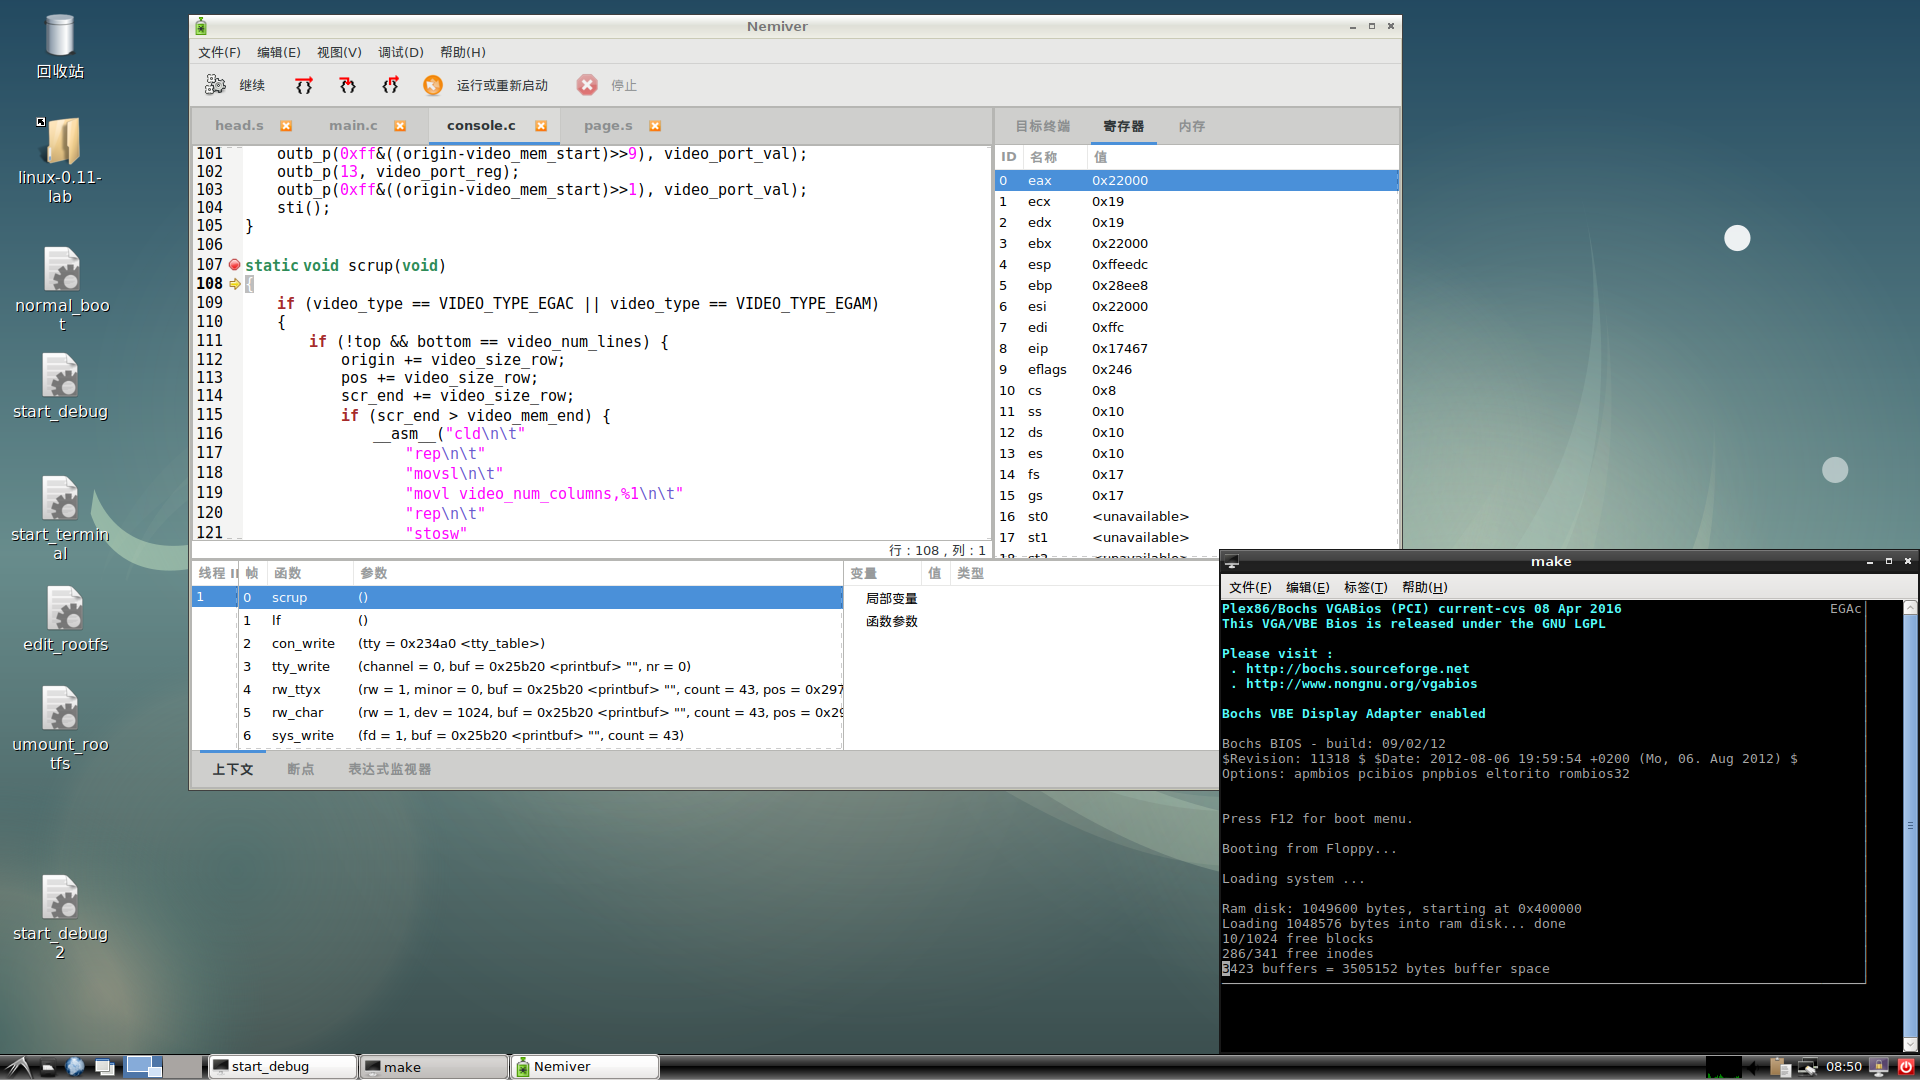
\includegraphics[width=0.9\linewidth]{img/1.png}
	\caption[]{gdb图形界面, 用于单步调试Linux 0.11}
	%\label{fig}
\end{figure}

\begin{figure}[htbp]
	\centering
	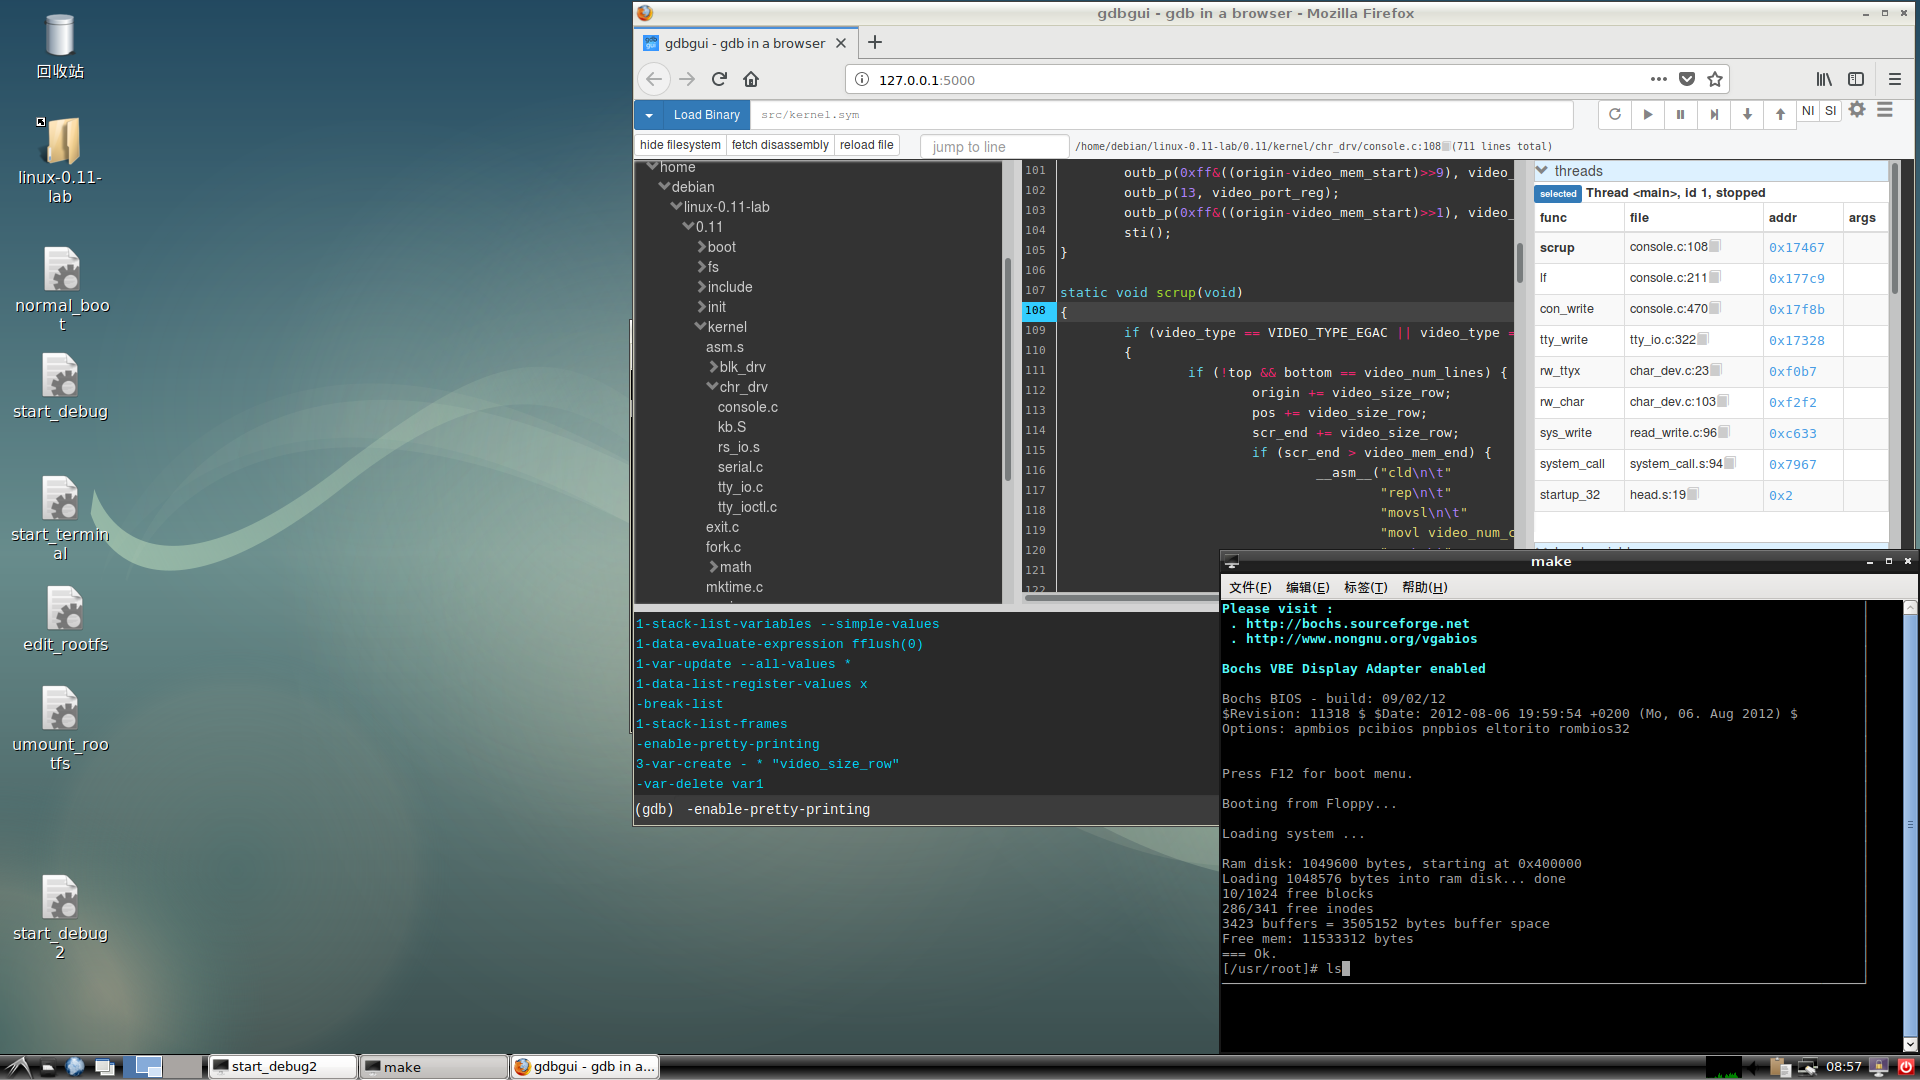
\includegraphics[width=0.9\linewidth]{img/2.png}
	\caption[]{gdb网页界面, 用于单步调试Linux 0.11}
	%\label{fig}
\end{figure}
\newpage
\begin{figure}[htbp]
	\centering
	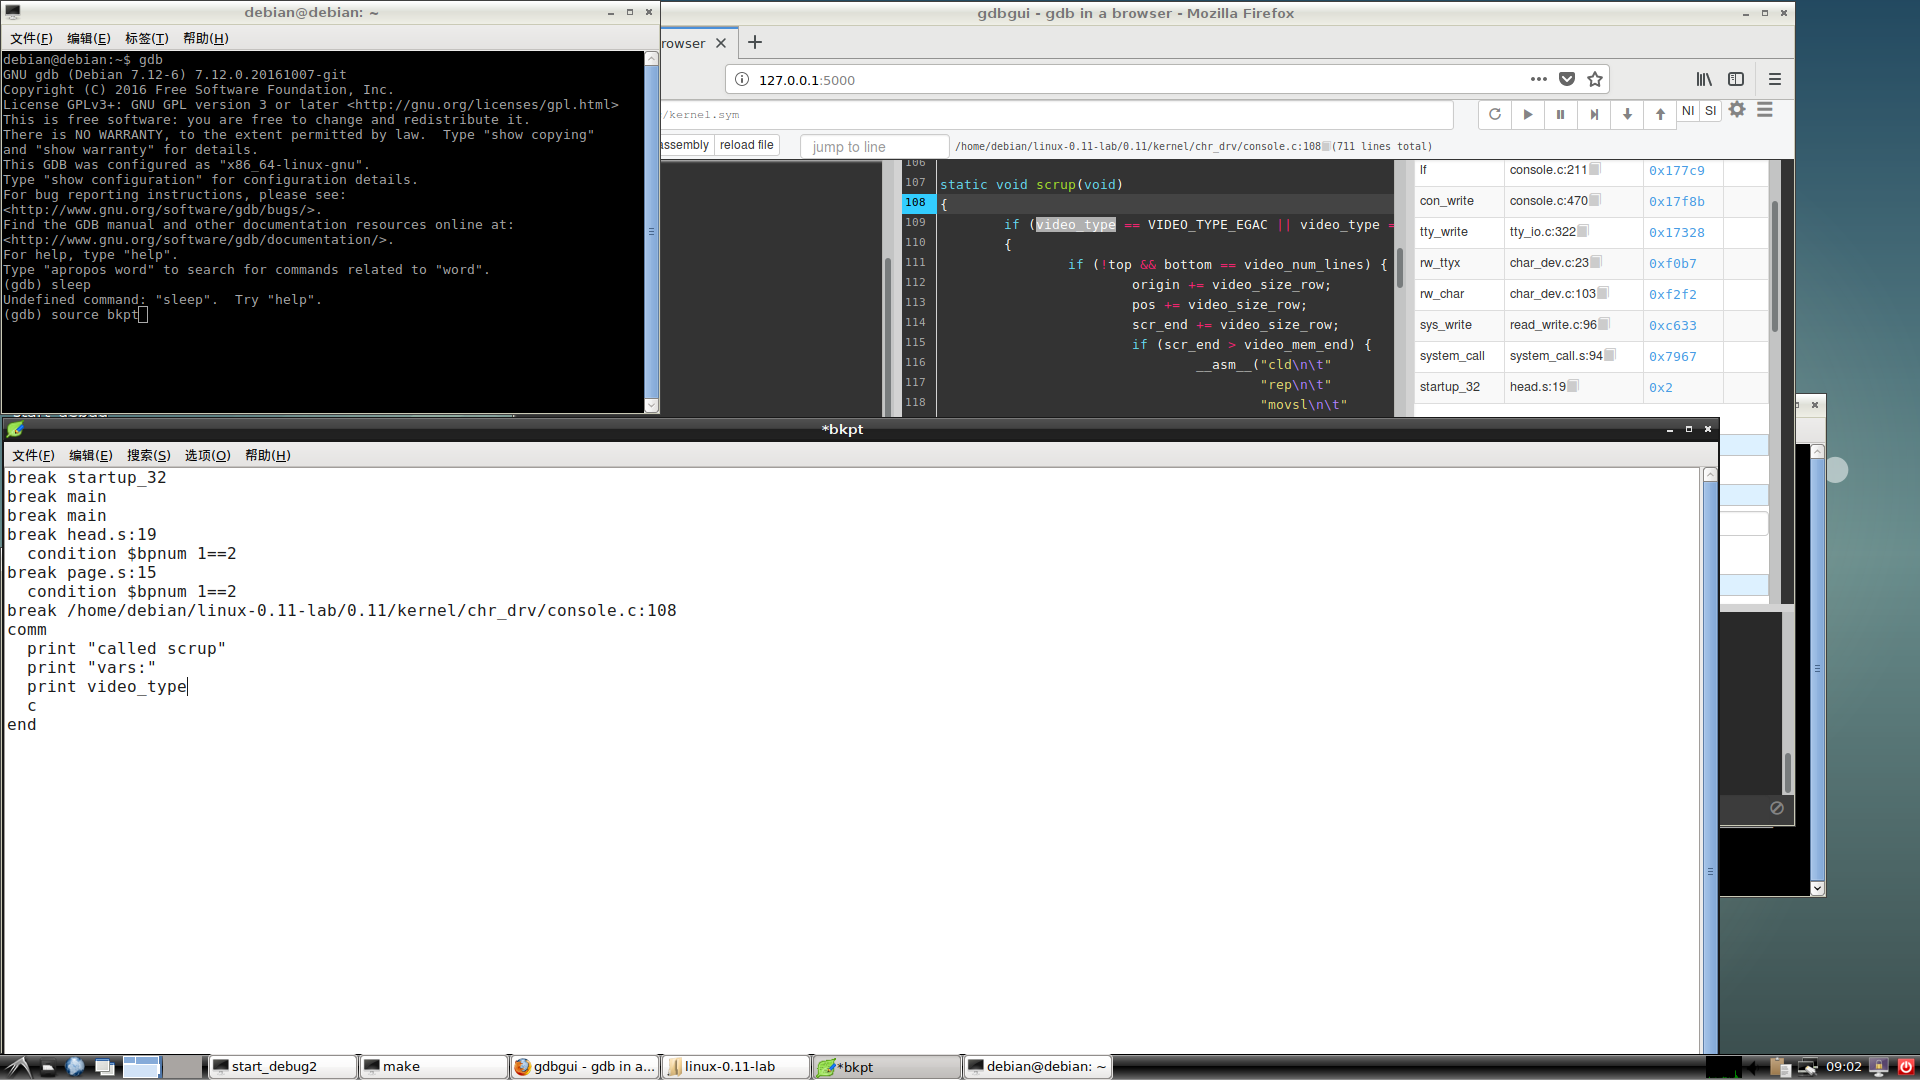
\includegraphics[width=0.9\linewidth]{img/3.png}
	\caption[]{使用gdb脚本调试}
	%\label{fig}
\end{figure}

\begin{figure}[htbp]
	\centering
	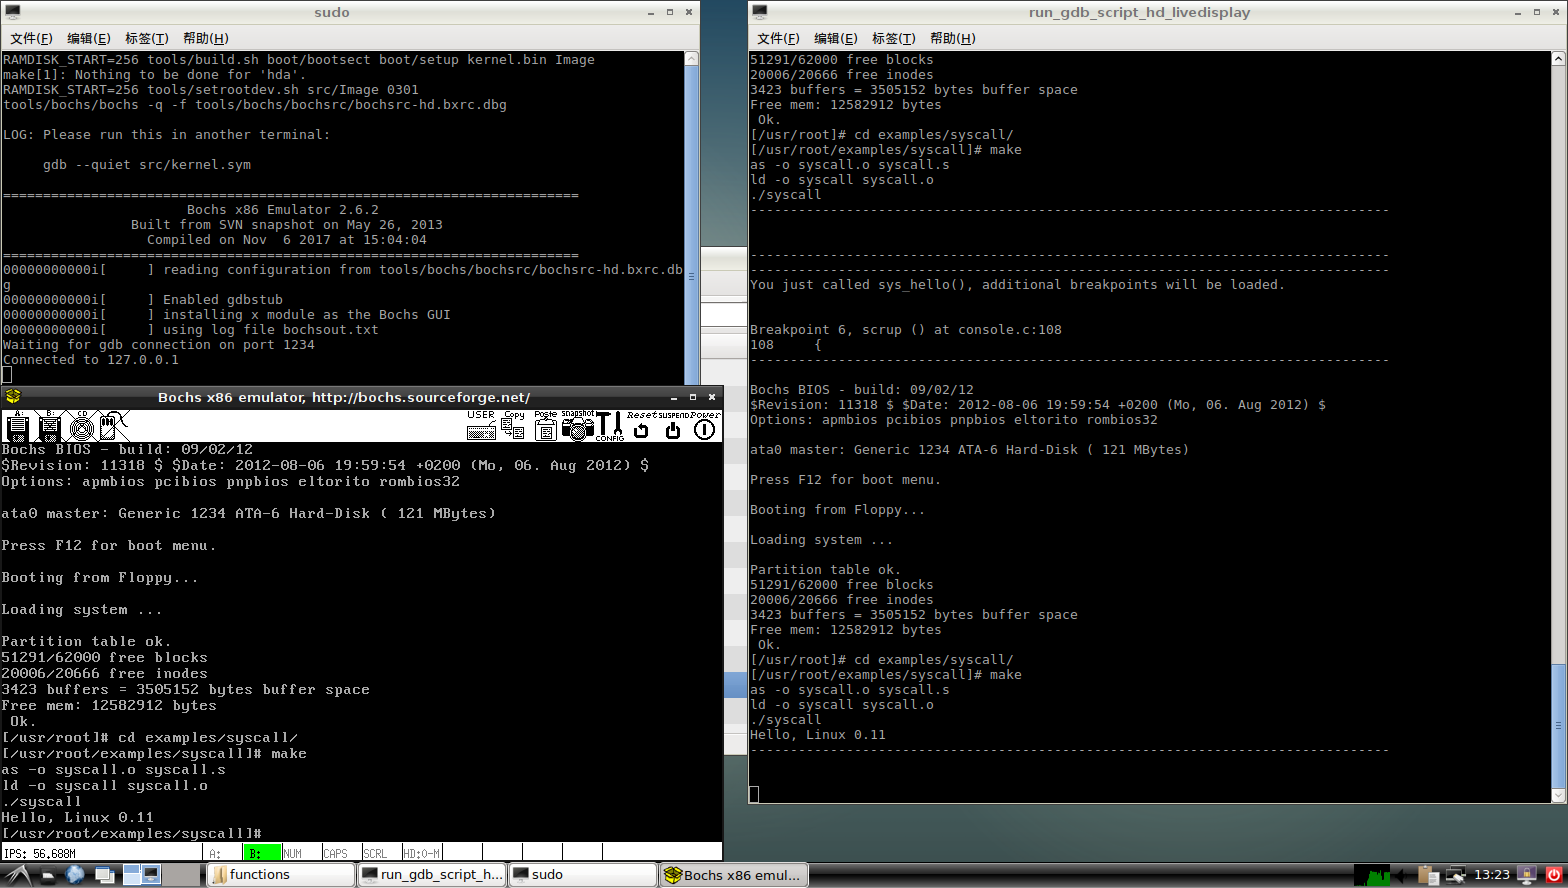
\includegraphics[width=0.9\linewidth]{img/4.png}
	\caption[]{执行系统调用syscall的过程}
	%\label{fig}
\end{figure}


\section{感想}
\subsection{不足之处}
\begin{enumerate}
	\item 由于时间原因, 动画效果不是特别精美;
	\item 个别时间, 存在同组两人一人忙, 另一人闲的情况;
	\item 本实验报告中, 引用格式不是特别规整;
	\item 可视化部分代码复用性较差.
\end{enumerate}
\subsection{收获}
\begin{enumerate}
	\item 对Linux 0.11有了进一步的认识, 加深了对操作系统课程内容的理解;
	\item 理解linux操作系统的基本工作原理;
	\item 对同步、异步有了更深的认识;
	\item 更加熟练地使用gdb调试脚本;
	\item 积累了JavaScript制作动图的经验;
	\item 积累了处理矢量图的经验, 本实验报告中一部分插图(包括可视化应用界面), 均为矢量图, 可在pdf阅读器中任意放大;
	\item 同陈宇翔同学合作的过程中, 加强了我们合作交流的能力.
\end{enumerate}
\subsection{对课程的建议}
\begin{enumerate}
	\item 建议同学们加强沟通与交流, 以实现合作互补. 我与陈宇翔同组, 陈宇翔学了汇编语言选修课, 专攻提取数据的方案; 我选了Web技术, 专攻可视化方案, 效果很好.
	\item 建议下一级同学阅读代码时, 不要太纠结于细节;
	\item 建议将提取数据的时间增加一周, 可视化的时间减少一周.
\end{enumerate}
\end{document}